\chapter{Linear regulation}
\section{Theory and related work} \label{sec:literature_linear}
Linear regulators behave like variable resistance devices, where the internal resistance is varied in order to maintain a constant output voltage. In reality, the variable resistance is provided by means of a transistor controlled by an amplifier feedback loop. They reject any input voltage ripple and are able to produce steady voltage outputs with very little noise. However, they are quite inefficient as they dissipate the difference between the input and output voltage as heat. Thus, they are a poor choice if the output voltage is much lower than the input voltage, as is the case in this design \cite{regulators-main}.


\section{Design} \label{sec:design_linear}
\textbf{\textit{Design rationale}}
As explained in Section \ref{sec:rationale_system}, the linear regulator is used to remove the noise produced by the switch-mode regulator. For efficient working of the linear regulator, the input voltage should not be too high. The maximum such voltage is calculated in Equation \ref{eq:linear_input} below.

The input and output capacitors are taken from the device datasheet \cite{LM7805}. The input capacitor is not included in the design since the input pin is connected to the output of the switch-mode regulator, that already has a $\SI{220}{\mu\farad}$ capacitor. This is much larger than the $\SI{330}{\nano\farad}$ specified. A $\SI{100}{\nano\farad}$ output capacitor is included to improve the transient response.


\noindent\textbf{\textit{Design calculations}} \\
\textit{Input voltage:}
\begin{equation*}
    \begin{split}
        P_{dissipated,max} &=  V_{in,max}I_{in} - V_{out}I_{load} \\
        P_{dissipated,max} &= \frac{T_{J,max} - T_{air}}{\Theta_{JA}} \\
        &=\frac{150-25}{150}=\SI{833.33}{\milli\watt} \\
    \end{split}
\end{equation*}
\begin{equation}
    \begin{split}
        V_{in,max} &= \frac{P_{dissipated,max} + V_{out}I_{load}}{I_{load}+I_Q} \\ 
        &=\frac{0.8333+(5 \times 100m)}{100m+2m} \\
        &=\SI{13.072}{\volt}
    \end{split}
    \label{eq:linear_input}
\end{equation}
A \SI{9.5}{\volt} input is chosen as it meets the above requirement as well as that of the charge pump in Section \ref{sec:design_chargepump}.
\\

\noindent\textbf{\textit{Circuit diagram}} \label{subsec:design_linear_circuit}
\begin{figure}[h]
 \centering
  	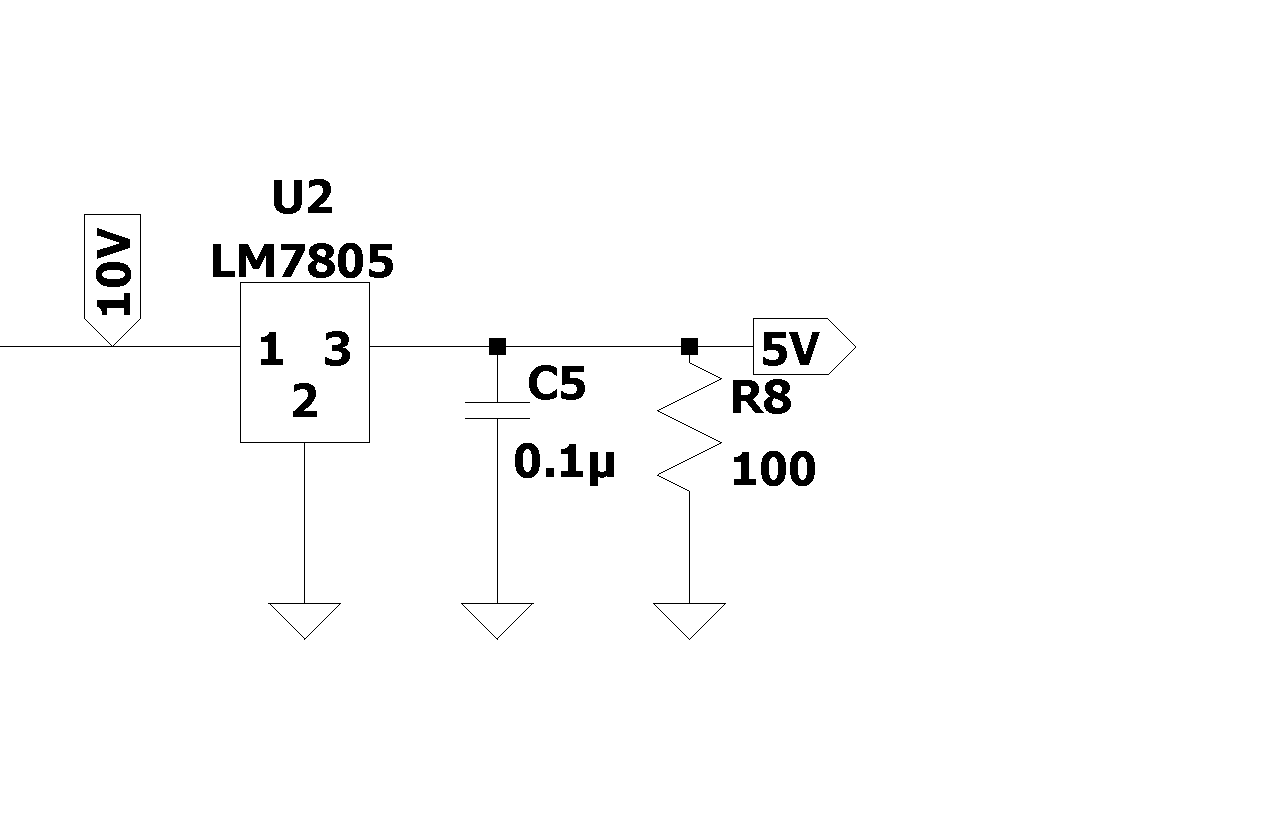
\includegraphics[width=0.75\linewidth,clip,trim = 0cm 3cm 0cm 3cm]{./Figures/linear_circuit.pdf}
  	\caption{Linear regulator circuit.}
  	\label{fig:linear_circuit}
 \end{figure}
 
 

\section{Simulation} \label{sec:simulation_linear}
A plot of the LTSpice linear regulation simulation is given in Figure \ref{fig:+5v_simulation}.

\begin{figure}[h] 
 \centering
  	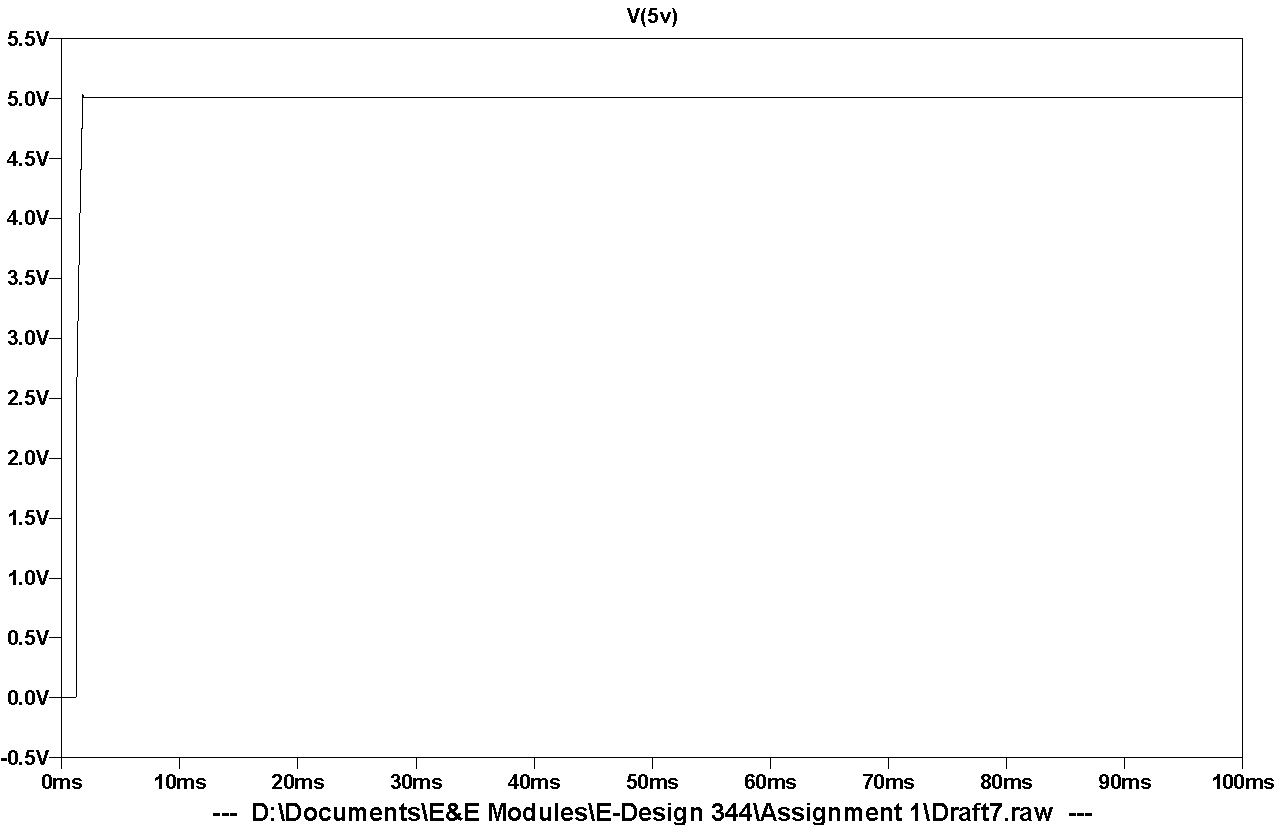
\includegraphics[width=0.7\linewidth]{./Figures/linear_simulate.pdf}
  	\caption{Simulated +5V output.}
  	\label{fig:+5v_simulation}
 \end{figure}
 
 
\section{Measurements} \label{sec:measurements_linear}
A plot of the measured output voltage from the linear rectifier is given in Figure \ref{fig:5v_measurement_box}. This contains both the DC voltage level (Figure \ref{fig:5v_output_measurement}) as well as the noise levels under AC coupling (Figure \ref{fig:5v_noise_measurement}).

\begin{figure}[h] 
 \centering
 
    \begin{subfigure}[]{0.49\linewidth}
        \centering
        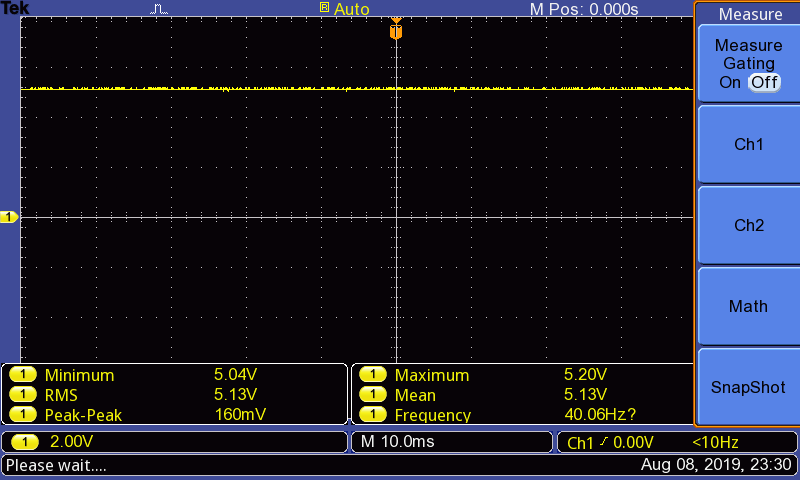
\includegraphics[width=1.\linewidth,clip,trim = 0cm 0cm 2.5cm 0cm]{./Figures/5v_test}
        \caption{+5V output voltage}
        \label{fig:5v_output_measurement}
    \end{subfigure}
    \begin{subfigure}[]{0.49\linewidth}
        \centering
        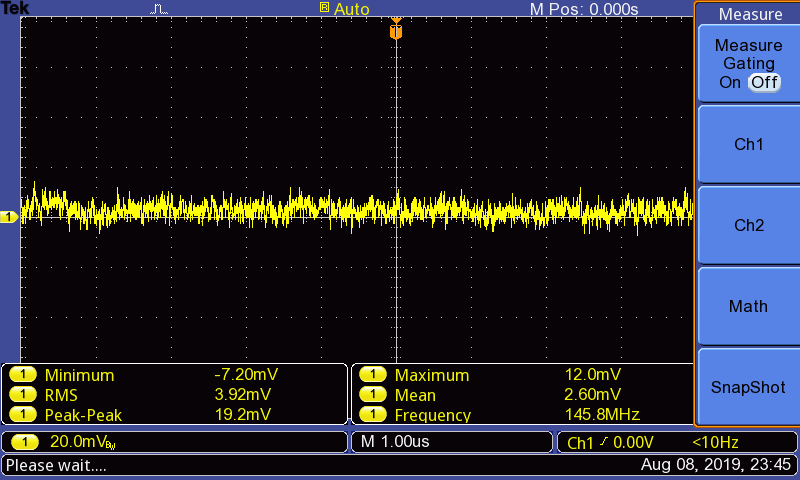
\includegraphics[width=1.\linewidth,clip,trim = 0cm 0cm 2.5cm 0cm]{./Figures/5v_noise_test}
        \caption{+5V noise levels.}
        \label{fig:5v_noise_measurement}
    \end{subfigure}
    
\caption{+5V measured output}
\label{fig:5v_measurement_box}
\end{figure}








